
\chapter{Diseño e implementación} % Main chapter title
En este capítulo se abordará la descripción de la arquitectura general del sistema, arquitectura del firmware, código de los controladores desarrollados, desarrollo del hardware y la configuración de la plataforma IoT.
\label{Chapter3} % Change X to a consecutive number; for referencing this chapter elsewhere, use \ref{ChapterX}

\definecolor{mygreen}{rgb}{0,0.6,0}
\definecolor{mygray}{rgb}{0.5,0.5,0.5}
\definecolor{mymauve}{rgb}{0.58,0,0.82}
\definecolor{mypurple}{rgb}{47,7,245}
%%%%%%%%%%%%%%%%%%%%%%%%%%%%%%%%%%%%%%%%%%%%%%%%%%%%%%%%%%%%%%%%%%%%%%%%%%%%%
% parámetros para configurar el formato del código en los entornos lstlisting
%%%%%%%%%%%%%%%%%%%%%%%%%%%%%%%%%%%%%%%%%%%%%%%%%%%%%%%%%%%%%%%%%%%%%%%%%%%%%
\lstset{ %
  backgroundcolor=\color{white},   % choose the background color; you must add \usepackage{color} or \usepackage{xcolor}
  basicstyle=\footnotesize,        % the size of the fonts that are used for the code
  breakatwhitespace=false,         % sets if automatic breaks should only happen at whitespace
  breaklines=true,                 % sets automatic line breaking
  captionpos=b,                    % sets the caption-position to bottom
  commentstyle=\color{mygreen},    % comment style
  deletekeywords={...},            % if you want to delete keywords from the given language
  %escapeinside={\%*}{*)},          % if you want to add LaTeX within your code
  %extendedchars=true,              % lets you use non-ASCII characters; for 8-bits encodings only, does not work with UTF-8
  %frame=single,	                % adds a frame around the code
  keepspaces=true,                 % keeps spaces in text, useful for keeping indentation of code (possibly needs columns=flexible)
  keywordstyle=\color{blue},       % keyword style
  language=[ANSI]C,                % the language of the code
  %otherkeywords={*,...},           % if you want to add more keywords to the set
  numbers=left,                    % where to put the line-numbers; possible values are (none, left, right)
  numbersep=5pt,                   % how far the line-numbers are from the code
  numberstyle=\tiny\color{mygray}, % the style that is used for the line-numbers
  rulecolor=\color{black},         % if not set, the frame-color may be changed on line-breaks within not-black text (e.g. comments (green here))
  showspaces=false,                % show spaces everywhere adding particular underscores; it overrides 'showstringspaces'
  showstringspaces=false,          % underline spaces within strings only
  showtabs=false,                  % show tabs within strings adding particular underscores
  stepnumber=1,                    % the step between two line-numbers. If it's 1, each line will be numbered
  stringstyle=\color{mymauve},     % string literal style
  tabsize=2,	                     % sets default tabsize to 2 spaces
  emph={sprintf, read_i2c_port_ExpectAndReturn,read_i2c_port_ReturnThruPtr_buffer
  ,TEST_ASSERT_EQUAL,send_data_ExpectAndReturn,aht10_launch_measurement}, 
  emphstyle=\color{violet},
  emph={[2]BG96_ERROR_SEND_SMS,BG96_ERROR_PUBLISH_MESSAGE,BG96_ERROR_CONNECT_SERVER_MQTT, RS_BG96_CERO,RF_ERROR,st_bg96_config,em_bg96_error_handling,AHT10_ADDRESS_SLAVE,int8_t,aht10_config_t,aht10_status_fnc,RS_SIG,RS_OK,RF_OK,RF_ERROR,uint8_t,SENSOR_BUSY,AHT10_OK,AHT10_ADDRESS,SENSOR_IDLE,AHT10_ERROR,uint32_t},emphstyle={[2]\color{blue}},
  emph={[3]obj,self},emphstyle={[3]\color{orange}},
  title=\lstname,                  % show the filename of files included with \lstinputlisting; also try caption instead of title
  morecomment=[s]{/*}{*/}
}


%----------------------------------------------------------------------------------------
%	SECTION 1
%----------------------------------------------------------------------------------------
\section{Diagrama de bloques general del sistema}

En la figura \ref{fig:Diagrama general del sistema IoT} se muestra el diagrama en bloques general del sistema donde se describe la arquitectura IoT aplicada al trabajo que consta de tres capas: percepción, red y aplicación.

\begin{figure}[h]
	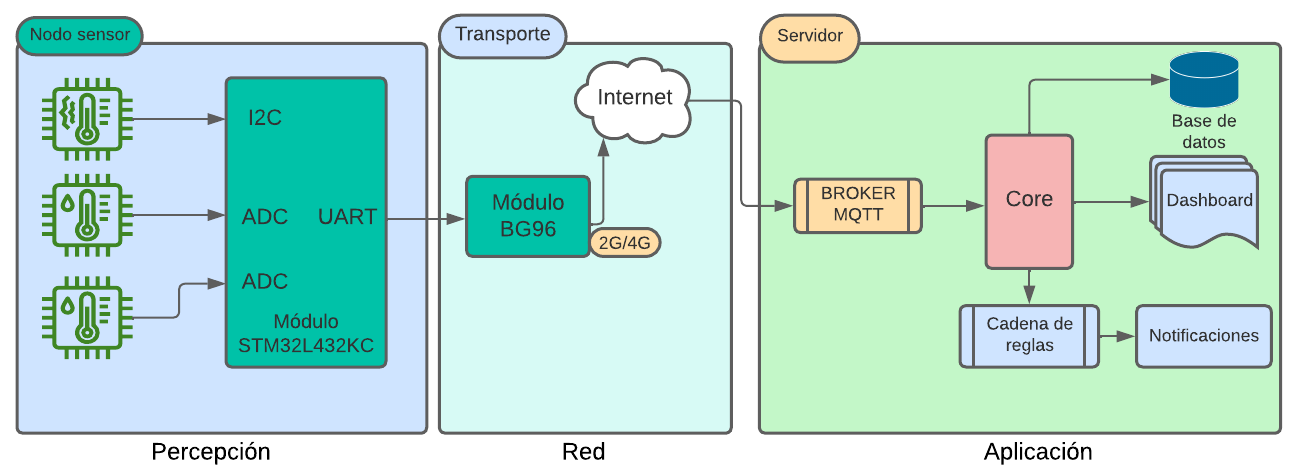
\includegraphics[width=\textwidth, height=8cm]{./Figures/DiagramaDelSistema.png}
	\caption{Diagrama general del sistema IoT.}
	\label{fig:Diagrama general del sistema IoT}
\end{figure}

En cada una de las capas se despliegan tecnologías y componentes de hardware y software. A continuación se describe cada una de las capas.

\begin{itemize}
	\item Capa de percepción: en la capa de percepción se encuentra el nodo sensor que es el encargado de medir las variables físicas, hacer un preprocesamiento y posteriormente enviar los datos a la capa de red. Para su desarrollo se utilizó la tarjeta de prueba STM32L432KC que contiene el firmware del sistema, además, se utilizaron los siguientes sensores: sensor de humedad y temperatura ambiente AHT10, sensor de humedad de suelo HL-69 y el sensor de luz UV ML8511.
  \item Capa de red: en lo que respecta a la conectividad de red, se empleó un módulo Quectel BG96 que es capaz de establecer conexión de manera automática con las redes 2G, 4G y NB-IoT, según las condiciones de red en el lugar de implementación del nodo sensor. Este módulo se comunica con el microcontrolador mediante comandos AT a través del puerto UART.
  \item Capa de aplicación: en la capa de aplicación, se utilizó ThingsBoard como plataforma IoT que brinda los microservicios de broker MQTT como puerta de entrada al servidor, base de datos para el almacenamiento, interfaz gráfica para la visualización de los datos y permite gestionar las alarmas del sistema.
\end{itemize}

\section{Arquitectura de firmware}
El desarrollo del firmware fue la tarea más compleja del trabajo debido a que uno de los objetivos fue lograr un firmware estructurado en capas para facilitar el desarrollo y reducir la complejidad del código. La figura \ref{fig:Capas del firmware} muestra la división en capas del firmware desarrollado.

\begin{figure}[h]
  \centering
	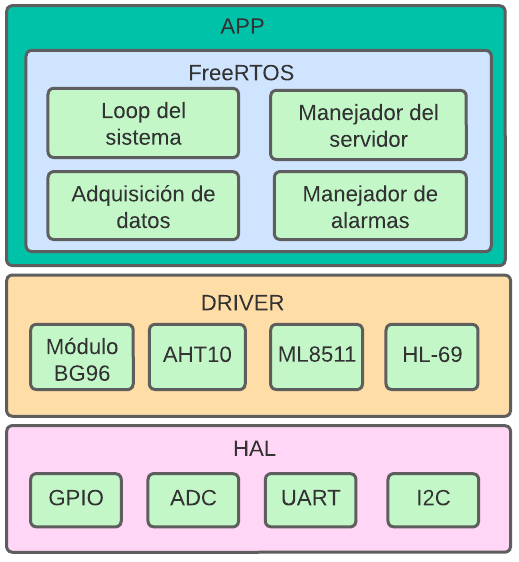
\includegraphics[width=7cm, height=8cm]{./Figures/Capas del firmware.png}
	\caption{Capas del firmware.}
	\label{fig:Capas del firmware}
\end{figure}

\subsection{Capa HAL} 
La capa HAL (\textit{Hardware Abstraction Layer}) proporcionada por el fabricante del microcontrolador  es la más baja del sistema, proporciona a las capas superiores la capacidad de interactuar con los periféricos del  microcontrolador a través de funciones en lenguaje C.
\begin{itemize}
  \item GPIO: la API proporciona funciones  para gestionar las entradas y salidas del microcontrolador. Fueron utilizadas por la capa de APP para el control de los leds de debug y para el encendido y reset del módulo de comunicación.
  \item ADC: proporcionan funciones para la configuración, lectura y escritura de los pines del microcontrolador para trabajar con señales analógicas. Se utilizaron estas funciones para hacer la lectura de los sensores de humedad del suelo y el sensor de luz UV.
  \item UART: brinda funciones para la lectura y escritura del puerto UART del microcontrolador. El firmware utiliza estas funciones para la comunicación con el módulo BG96.
  \item I2C: proporciona funciones para la lectura y escritura por protocolo I2C. El driver del sensor AHT10 utiliza estas funciones para hacer la lectura de los datos.
\end{itemize}

\subsection{Capa drivers} 
La capa drivers (manejador de dispositivos) está compuesta por los manejadores que se desarrollaron para interactuar con el hardware externo al microcontrolador. Se desarrollaron dos drivers que se describen a continuación:
\begin{itemize}
  \item Driver BG96: las funciones más importantes que proporciona el driver son:
  \begin{itemize}
    \item Estado del módulo.
    \item Descripción del módulo.
    \item Configuración APN de la red.
    \item Conexión TCP.
    \item Conexión al broker MQTT.
  \end{itemize}
  \item Driver AHT10: se desarrolló utilizando la hoja de datos del sensor, proporciona funciones de inicialización y lectura de humedad y temperatura obtenidos por el sensor.
\end{itemize}
Para los sensores ML8511 y HL-69 que son sensores analógicos no se desarrollaron drivers, sino que se crearon funciones para convertir el valor analógico entregado a un valor significativo para el usuario con respecto a la variable física medida.
\subsection{Capa aplicación} 
La capa de APP o aplicación  es la de mayor nivel jerárquico. Se desarrolló sobre freeRTOS 
que permite hacer un código más escalable.

Se implementaron cuatro tareas, que se describen a continuación:
\begin{itemize}
    \item Loop del sistema: esta tarea es la que brinda la secuencialidad del sistema.
    \item Manejador del  servidor: se encarga de manejar la conexión a la red y al broker MQTT.
    \item Adquisición de datos: se encarga de hacer la lectura de los sensores.
    \item Manejador de alarmas: esta tarea se encarga de hacer el control de las alarmas del sistema.
\end{itemize}
\clearpage

\section{Desarrollo del firmware}

Para el desarrollo del firmware se utilizó STM32CubeIDE que es el entorno de desarrollo oficial de STMicroelectronic.

El firmware fue desarrollado sobre freeRTOS, se utilizaron algunas de sus funcionalidades como colas, semáforos, tareas e interrupciones.

En la figura \ref{fig:Df inicio firmware}  se muestra en diagrama de flujo de inicialización del firmware.

\begin{figure}[htbp]
  \centering
	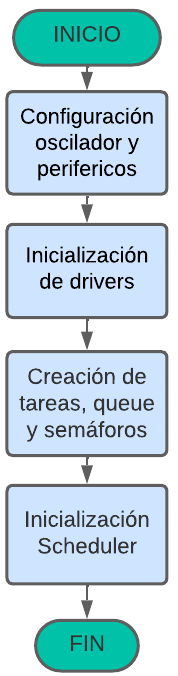
\includegraphics[width=2.5cm, height=9.5cm]{./Figures/DF inicio firmware.png}
	\caption{Diagrama de flujo de inicialización del firmware.}
	\label{fig:Df inicio firmware}
\end{figure}

El firmware comienza realizando la siguiente secuencia de acciones: configuración del hardware del microcontrolador, inicialización de los drivers del hardware externo, creación de los recursos del sistema operativo y finalmente inicialización del scheduler.

Para el control del sistema se crearon cuatro tareas sobre freeRTOS, que se comunican y sincronizan a través de colas y semáforos.

\subsection{Tarea loop del sistema} 

La tarea loop es un bucle que se encarga de brindar la secuencialidad al firmware, manda eventos a las demás tareas para que sean procesados. 

Comienza iniciando un timer que se encarga controlar el tiempo de repetición del ciclo de la tarea. Luego la tarea se bloquea. 
Cuando se termina el tiempo del timer, se ejecuta el handler de la interrupción desbloqueando la tarea loop. La tarea envía un evento a la cola de adquisición de datos para realizar la lectura  de  los sensores y un evento a la cola que maneja la conexión  para levantar el servidor. Posteriormente la tarea comprueba si se logró levantar una conexión. Si la conexión existe la tarea manda un evento  por la cola del servidor para que se envíen los datos al broker MQTT. Luego la tarea  envía un evento a la cola de alarmas para mandar los SMS (Short Message Service) de las alarmas activas del sistema. Finalmente, después de monitorear  las alarmas la tarea manda un evento a la cola de servidor para la desconexión. Al finalizar el ciclo de la tarea, inicia el timer nuevamente y manda al microcontrolador a modo de bajo consumo para ahorrar energía.

\begin{figure}[h]  
\centering
	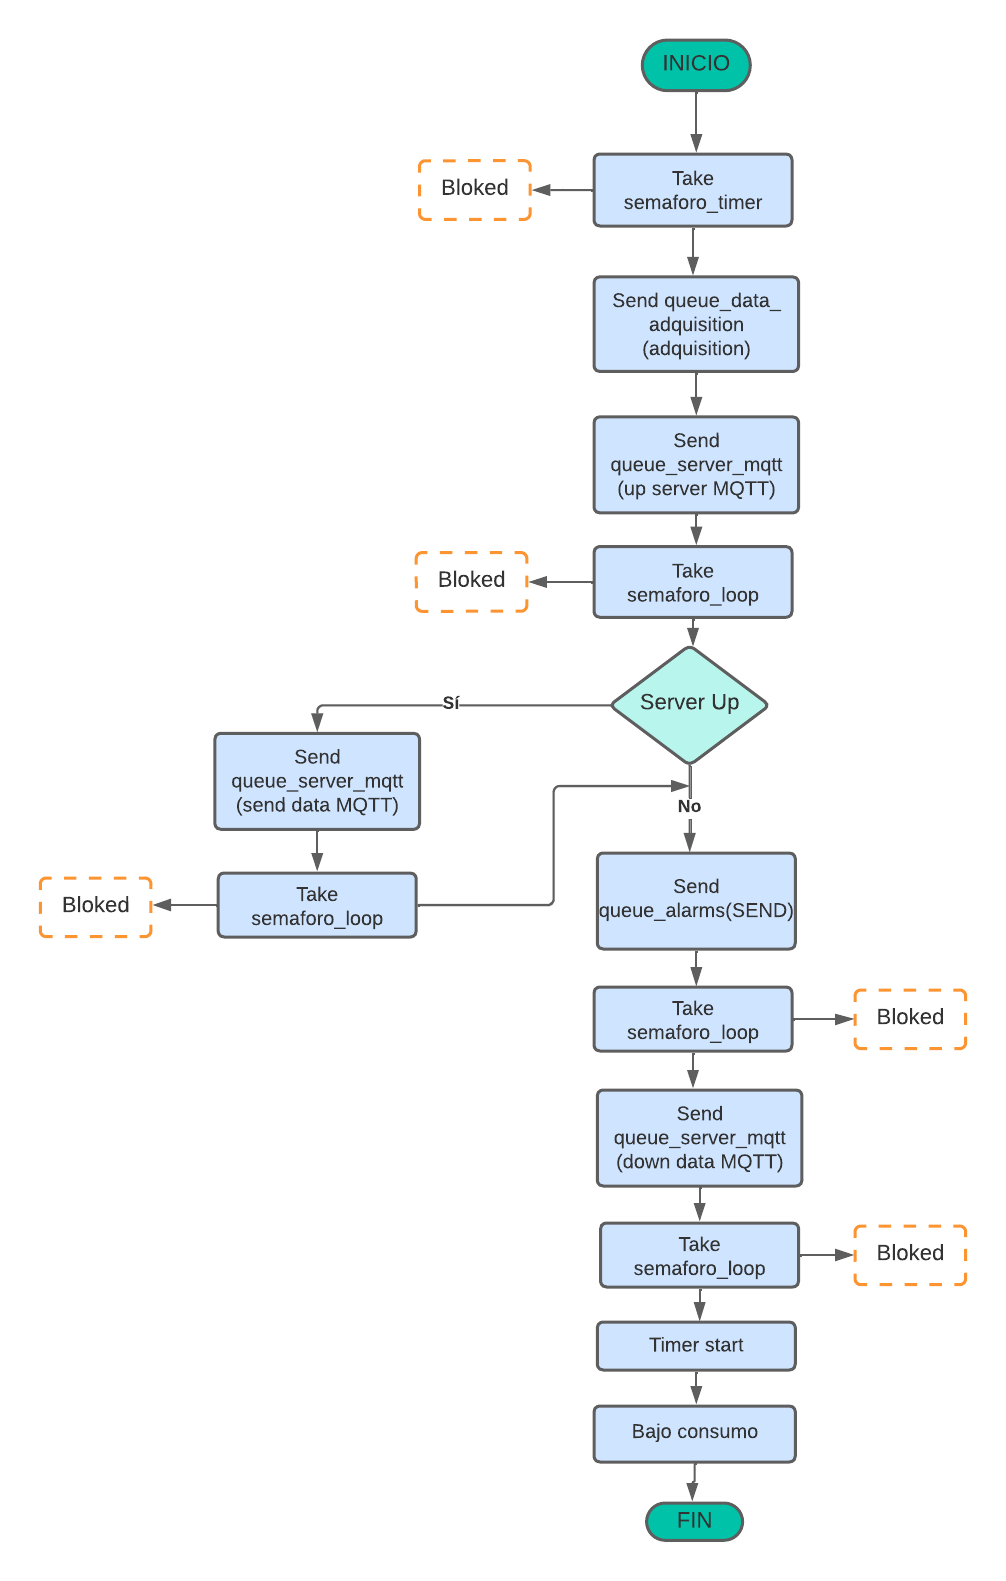
\includegraphics[width=12cm, height=16cm]{./Figures/DF task loop.png}
	\caption{Diagrama de flujo de la tarea loop.}
	\label{fig:Df tarea loop sistema}
\end{figure}

\subsection{Tarea adquisición de datos} 
La tarea de adquisición de datos es la encargada de hacer la lectura de los sensores. La figura \ref{fig:Df tarea adquisicion} muestra el diagrama de flujo de la tarea. 

La tarea inicia revisando si hay datos en la cola de adquisición. Si existen datos se realiza la lectura de todos los sensores, para posteriormente enviar los  valores leídos por la cola de datos y alarmas. Si no hay datos en la cola la tarea se bloquea. 

\begin{figure}[h]
  \centering
	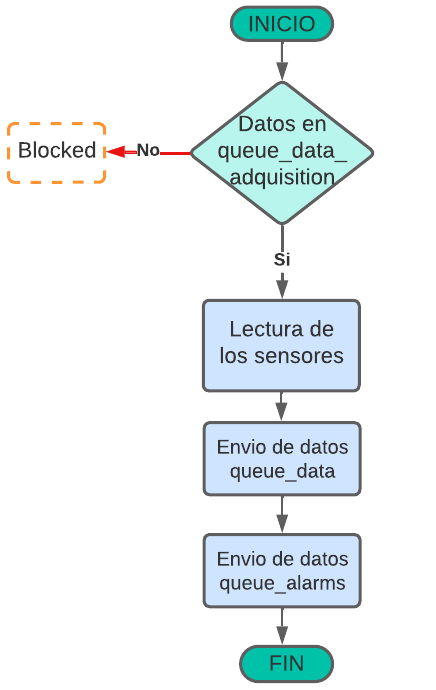
\includegraphics[width=5cm, height=7cm]{./Figures/DF task adquisicion.png}
	\caption{Diagrama de flujo tarea de adquisición de datos.}
	\label{fig:Df tarea adquisicion}
\end{figure}

\vspace{5cm}
\subsection{Tarea manejador de alarmas} 

Es la tarea encargada de monitorear que los valores leídos por los sensores no sean menores o mayores a los límites permitidos para la variable. La tarea activa una alarma si existe un valor fuera de los límites. La figura \ref{fig:Df tarea alarmas} muestra el diagrama de flujo de la tarea que maneja las alarmas.

Al ingresar al bucle infinito, la tarea comienza por inspeccionar la cola de alarmas. Si se encuentran datos en dicha cola, procede a analizar el evento que contiene la información recibida.

Existen dos tipos posibles de eventos: ``monitorear'' y  ``enviar''. En caso de que el evento sea ``monitorear'', se verifica si el valor del sensor de humedad es menor a 10. En caso afirmativo, se incrementa en uno la variable que lleva el registro de las alarmas activas. Si, por otro lado, el evento es ``enviar'', se verifica si existen alarmas activas y, de ser así, se envía un mensaje de texto.

En caso de no haber datos en la cola de alarmas, la tarea entra en un estado de bloqueo.

\begin{figure}[h]
  \centering
	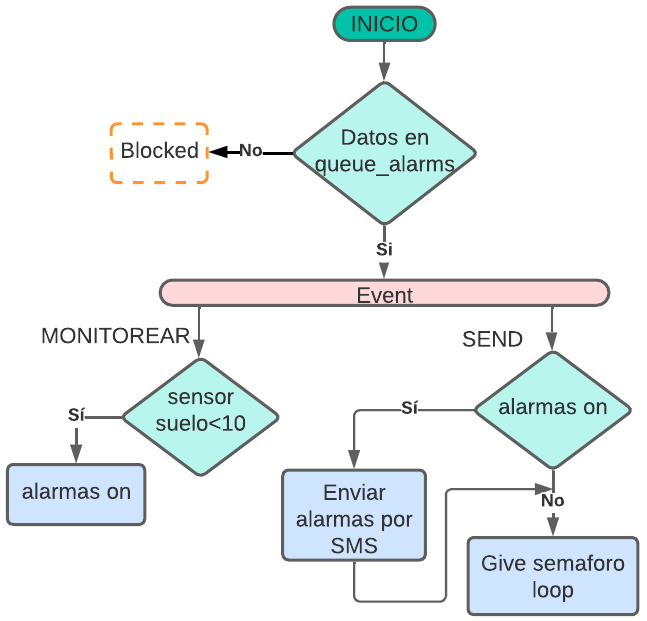
\includegraphics[width=6cm, height=6cm]{./Figures/DF_alarms.png}
	\caption{Diagrama de flujo de la tarea manejador de alarmas.}
	\label{fig:Df tarea alarmas}
\end{figure}

\subsection{Tarea manejador del servidor } 
La tarea se encarga de configurar, conectar y desconectar una conexión con el servidor. También permite enviar datos al broker MQTT. 

Comienza esperando datos en la cola del servidor, al llegar datos se analiza el evento que se recibe. Se tiene tres posibles eventos: UP, DOWN y SEND. Si el evento es UP, la tarea ingresa a la máquina de estados que se muestra en la figura \ref{fig:Maquina de estados up servidor}, la que se encarga de establecer una conexión con el servidor. Si el evento es DOWN, la tarea ejecuta la máquina de estados que se ve en la figura \ref{fig:Maquina de estados dowm servidor}, que se encarga de terminar la conexión con el servidor. Si el evento es SEND, la tarea obtiene los últimos datos leídos por los sensores, arma la trama y publica los datos al broker MQTT. 
\begin{figure}[h]
  \centering
	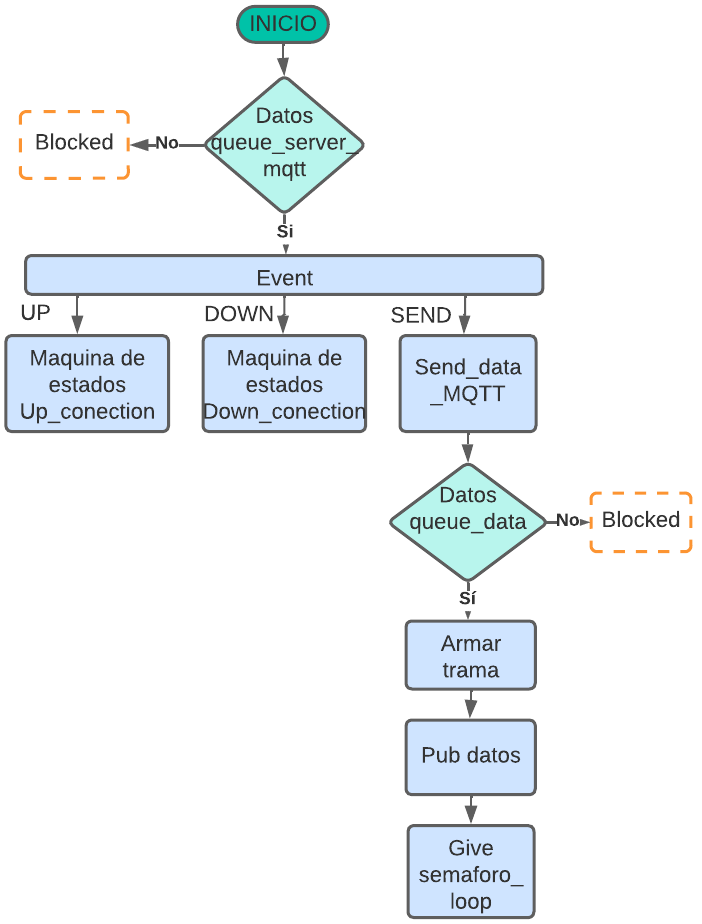
\includegraphics[width=8cm, height=8.1cm]{./Figures/DF general task conection.png}
	\caption{Diagrama de flujo de la tarea conexion server MQTT.}
	\label{fig:Df tarea conexion}
\end{figure}

\begin{figure}[h]
  \centering
  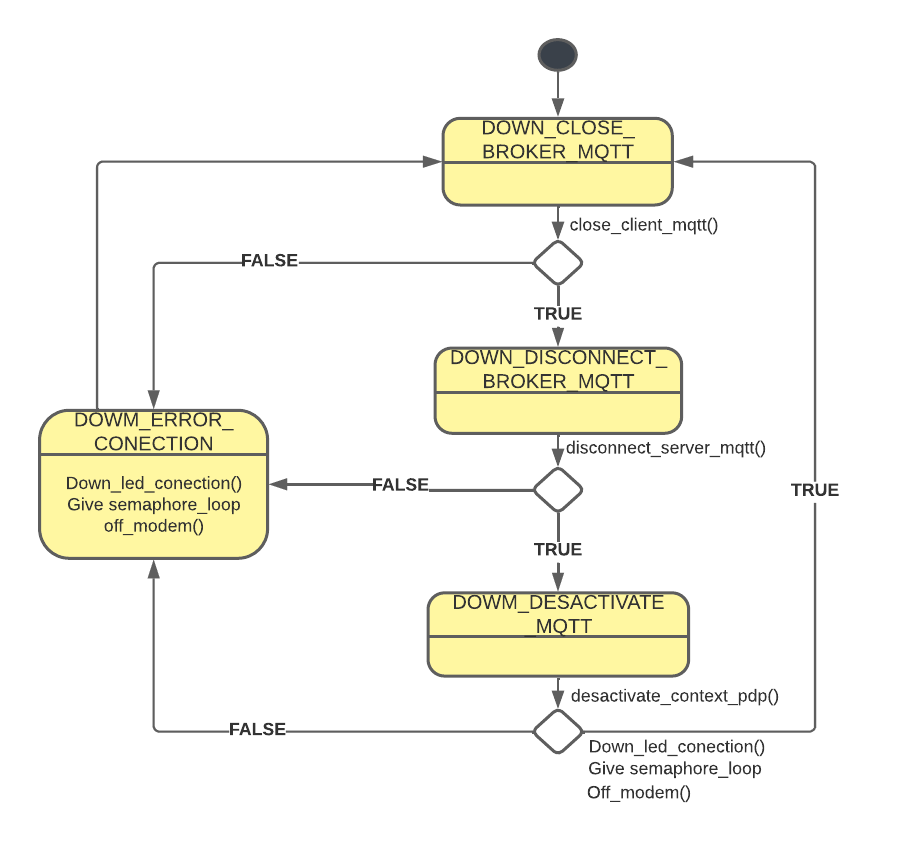
\includegraphics[width=8cm, height=7.7cm]{./Figures/SM down server.png}
  \caption{Máquina de estados down servidor.}
  \label{fig:Maquina de estados dowm servidor}
\end{figure}
\clearpage

\begin{figure}[t!]
  \centering
	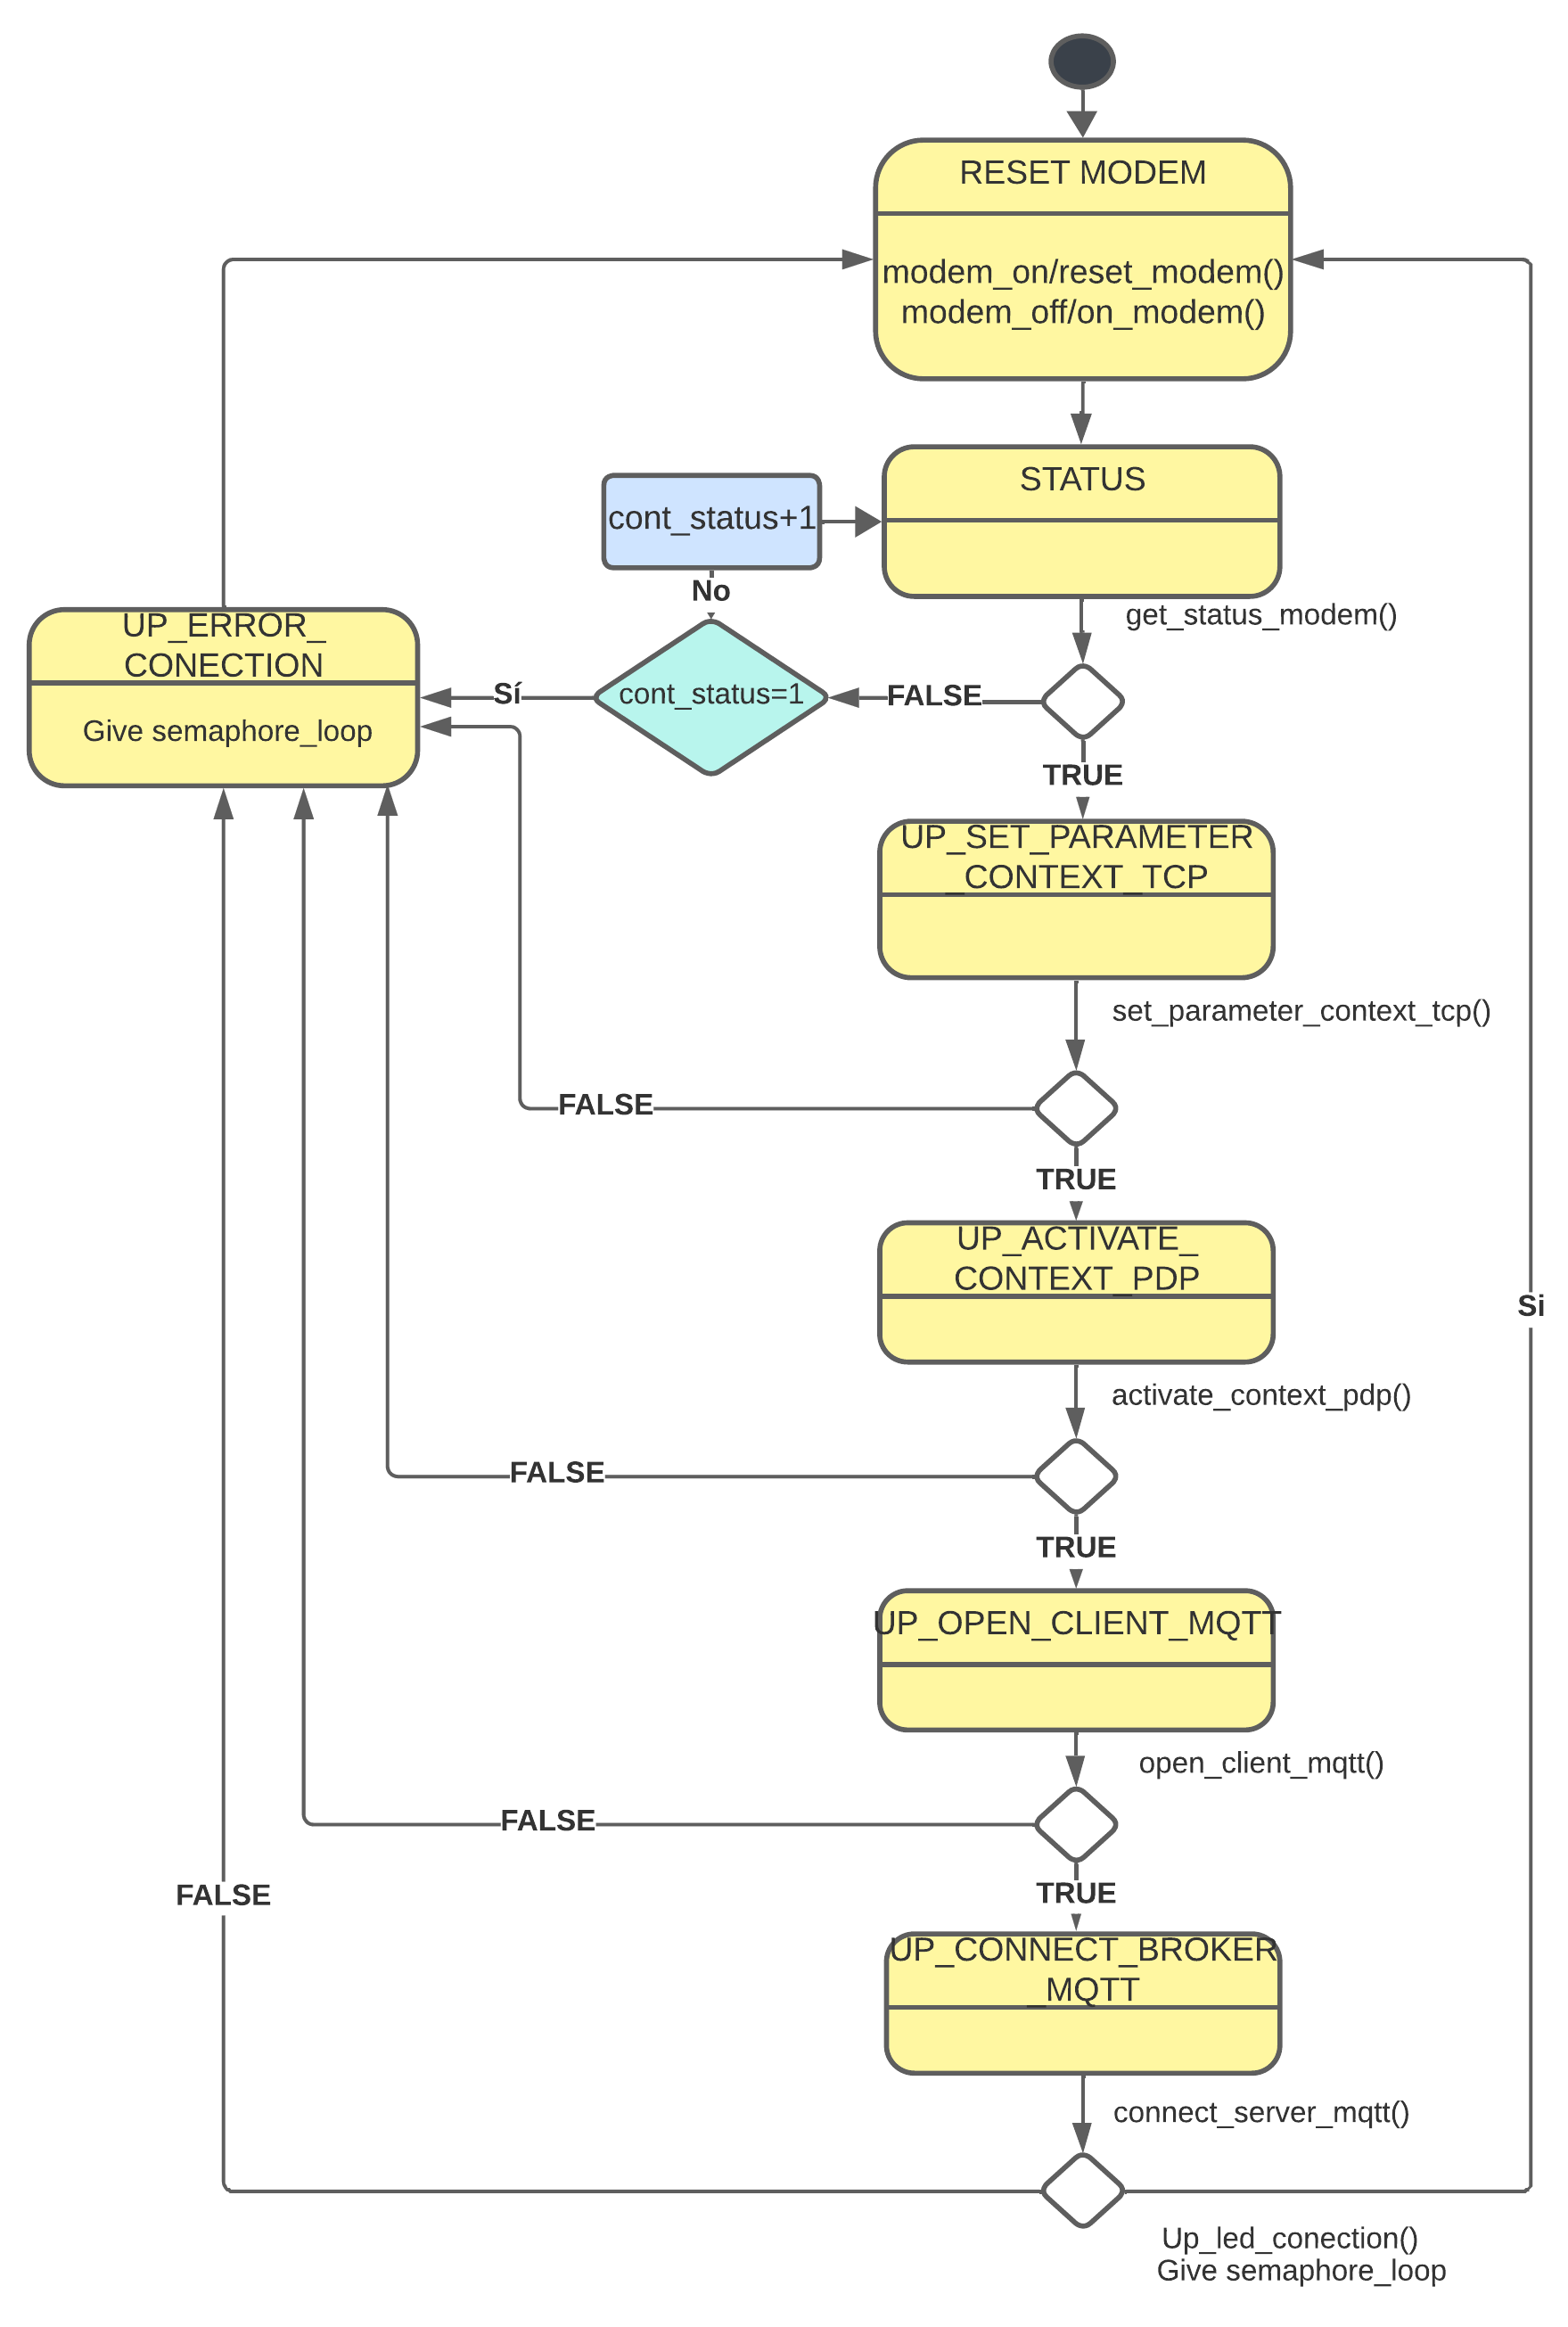
\includegraphics[width=10cm, height=13cm]{./Figures/SM up server.png}
	\caption{Máquina de estados up servidor.}
	\label{fig:Maquina de estados up servidor}
\end{figure}

\section{Controladores implementados}
Se implementaron dos controladores: para el módulo de comunicación BG96 y para el sensor de humedad y temperatura ambiente AHT10.

\subsection{Controlador para el sensor AHT10} 

Para la lectura de humedad y temperatura, se desarrolló en el driver las funciones de \emph{aht10\_get\_humedity()} y \emph{aht10\_get\_temperature()} que se muestran en el código \ref{cod:codigo funciones lectura}.
Las funciones comienzan iniciando una medición en el sensor con la función \emph{aht10\_launch\_measurement()}, luego realizan la lectura de los registros del sensor, almacenando los valores de retorno en un buffer. Con los bytes obtenidos se realiza un corrimiento para  obtener los bytes que contienen la información de humedad y temperatura. Finalmente, se aplican las fórmulas de las líneas 1 y 2 del código \ref{cod:codigo funciones lectura} para convertir los bytes en valores significativos de las variables físicas.
\begin{lstlisting}[label=cod:codigo funciones lectura ,caption=Funciones de lectura de humedad y temperatura.]  % Start your code-block

#define TEMPERATURE(A)                       (int8_t) ((A *0.000191)-50)       
#define HUMEDITY(A)                          (uint8_t) (A *0.000095)        
/**
 * @brief funcion para obtener el valor de la humedad
 * 
 * @param obj  puntero a la estructura principal del driver 
 * @param data puntero a la variable donde se retorna la humedad
 * @return aht10_status_fnc 
 */
aht10_status_fnc aht10_get_humedity(aht10_config_t*obj, uint8_t *data)
{
  obj->status_fun=AHT10_ERROR;
  uint8_t bufferRead[6]={0};
  uint32_t data_humedity=0;
  obj->status_fun=aht10_launch_measurement(obj);
  if (obj->status_fun==AHT10_OK)
  {
    obj->status_fun= obj->readI2C(AHT10_ADDRESS,bufferRead,6);
    if (obj->status_fun==AHT10_OK)
    {
      data_humedity=(((uint32_t)bufferRead[1]<<16) | ((uint16_t)bufferRead[2]<<8) | (bufferRead[3]))>>4;
      *data= HUMEDITY(data_humedity);
    }
  }
  return obj->status_fun;
}

/**
 * @brief funcion para obtener el valor de la temperatura
 * 
 * @param obj puntero a la estructura principal del driver 
 * @param data puntero a la variable donde se retorna la temperatura
 * @return aht10_status_fnc 
 */
aht10_status_fnc aht10_get_temperature(aht10_config_t*obj, int8_t *data)
{
  uint8_t buffer_read[6]={0};
  uint32_t data_temperature=0;
  obj->status_fun=AHT10_ERROR;
  obj->status_fun=aht10_launch_measurement(obj);
  if (obj->status_fun==AHT10_OK)
  {
    obj->status_fun=obj->readI2C(AHT10_ADDRESS ,buffer_read,6);
    if (obj->status_fun==AHT10_OK)
    {
      data_temperature=((uint32_t)(buffer_read[3] & 0x0F)<<16) | ((uint16_t) buffer_read[4]<<8)| buffer_read[5];
      *data= TEMPERATURE(data_temperature);
    }
  }
  return obj->status_fun;
}
\end{lstlisting}

\subsection{ Controlador para el módulo de comunicación BG96 } 
Se han creado diversas funciones destinadas al controlador BG96, las que posibilitan la configuración del módulo, la configuración de la red, y las más cruciales para el funcionamiento: las relacionadas con la conexión, publicación y desconexión del servidor MQTT.

El código \ref{cod:driver bg96} presenta dos funciones implementadas en el controlador BG96. La función \emph{connect\_server\_mqtt()} se emplea para establecer la conexión con el servidor MQTT. En su interior, esta función envía el comando visible en la línea 11 y aguarda la respuesta del módulo, que puede ser \emph{OK} o \emph{ERROR}.

La función \emph{publish\_message()} es una de las más utilizadas por el firmware, es la encargada de publicar la trama JSON que contiene los datos de los sensores al tópico configurado inicialmente. 
\begin{lstlisting}[label=cod:driver bg96,caption=Función de conexión y publicación al broker MQTT.]  % Start your code-block

/**
 * @brief funcion para conectarse al servidor MQTT
 * 
 * @param self puntero a la estructura principal del driver
 * @return em_bg96_error_handling 
 */
em_bg96_error_handling connect_server_mqtt(st_bg96_config *self)
{
  self->ft_resp=RF_ERROR;
  char cmd[150]={0};
  sprintf(cmd,"AT+QMTCONN=%u,\"%s\",\"%s\",\"%s\"\r",self->self_mqtt.identifier_socket_mqtt,self->self_mqtt.mqtt_client_id,self->self_mqtt.mqtt_username,self->self_mqtt.mqtt_password);
  self->ft_resp=self->send_data_device(cmd,RS_BG96_CERO,self->buffer_resp,10000);
  if (self->ft_resp!=RF_OK)
  {
    self->last_error=BG96_ERROR_CONNECT_SERVER_MQTT;
  }
  return self->ft_resp;
}

/**
 * @brief funcion para publicar un mensaje a un topico
 * 
 * @param self puntero a la estructura principal del driver
 * @param topic topico donde se mandaran los datos 
 * @param data datos a publicar
 * @return em_bg96_error_handling 
 */
em_bg96_error_handling publish_message(st_bg96_config *self,char *topic,char *data)
{
  self->ft_resp=RF_ERROR;
  char cmd[50]={0};
  char buffer_data[220]={0};
  sprintf(buffer_data,"%s\x1a\r",data);
  sprintf(cmd,"AT+QMTPUB=%u,0,0,0,\"%s\"\r",self->self_mqtt.identifier_socket_mqtt,topic);
  self->ft_resp=self->send_data_device(cmd,RS_SIG,self->buffer_resp,3000);
  if (RF_OK==self->ft_resp)
  {
    self->ft_resp=self->send_data_device(buffer_data,RS_BG96_CERO,self->buffer_resp,15000);
    if (self->ft_resp!=RF_OK)
    {
       self->last_error=BG96_ERROR_PUBLISH_MESSAGE;
    }   
  }
  else self->last_error=BG96_ERROR_PUBLISH_MESSAGE;
  return self->ft_resp;
}
\end{lstlisting}


Para el envío de mensajes de texto se desarrolló en el driver la función \emph{send\_sms\_bg96()} que recibe como parámetros el número al que se desea mandar el mensaje y el texto del mensaje a enviar. El firmware utiliza esta función para mandar mensajes de alarma al usuario.
El código \ref{cod:funcion de sms} muestra la implementación de la función \emph{send\_sms\_bg96()}
\begin{lstlisting}[label=cod:funcion de sms,caption=Función para enviar SMS.]  % Start your code-block

/**
 * @brief funcion para enviar mensajes de texto
 * 
 * @param self puntero a estructura principal del driver
 * @param number numero de telefono al que se mandara el mensaje
 * @param message mensaje de texto
 * @return em_bg96_error_handling 
 */
em_bg96_error_handling send_sms(st_bg96_config *self,char*number,char*message)
{
  self->ft_resp=RF_OK;
  char buffer_message[20];
  char buffer_number[20];
  sprintf(buffer_number,"AT+CMGS=\"%s\"\r",number);
  sprintf(buffer_message,"%s\x1a\r",message);
  self->ft_resp=self->send_data_device(buffer_number,RS_SIG,self->buffer_resp,12000);
  if (RF_OK==self->ft_resp)
  {
    self->ft_resp=self->send_data_device(buffer_message,RS_OK,self->buffer_resp,12000);
    if (RF_OK!=self->ft_resp)
    {
      self->last_error=BG96_ERROR_SEND_SMS;
    }
  }
  return self->ft_resp;
}
\end{lstlisting}

\section{Desarrollo del hardware}

Para el diseño del hardware se empleó KiCad 6.0, una herramienta de diseño que se utilizó durante el desarrollo de la especialización.

\subsection{Esquemático} 
Dado que se trata de un prototipo, se diseñó una tarjeta que permite la integración y conexión de los componentes utilizados en el trabajo, incluyendo el módulo de comunicación celular, la tarjeta de desarrollo con el microcontrolador y los módulos sensores.

En la figura \ref{fig:esquematico root} se muestra la página raíz del esquemático del trabajo, está dividida en tres zonas:
\begin{itemize}
  \item Zona 1: índice de las hojas esquemáticas del trabajo.
  \item Zona 2: modelo 3D de la tarjeta desarrollada.
  \item Zona 3: conexiones entre los diferentes hojas esquemáticas .
\end{itemize}
\clearpage

\begin{figure}[h]
  \centering
	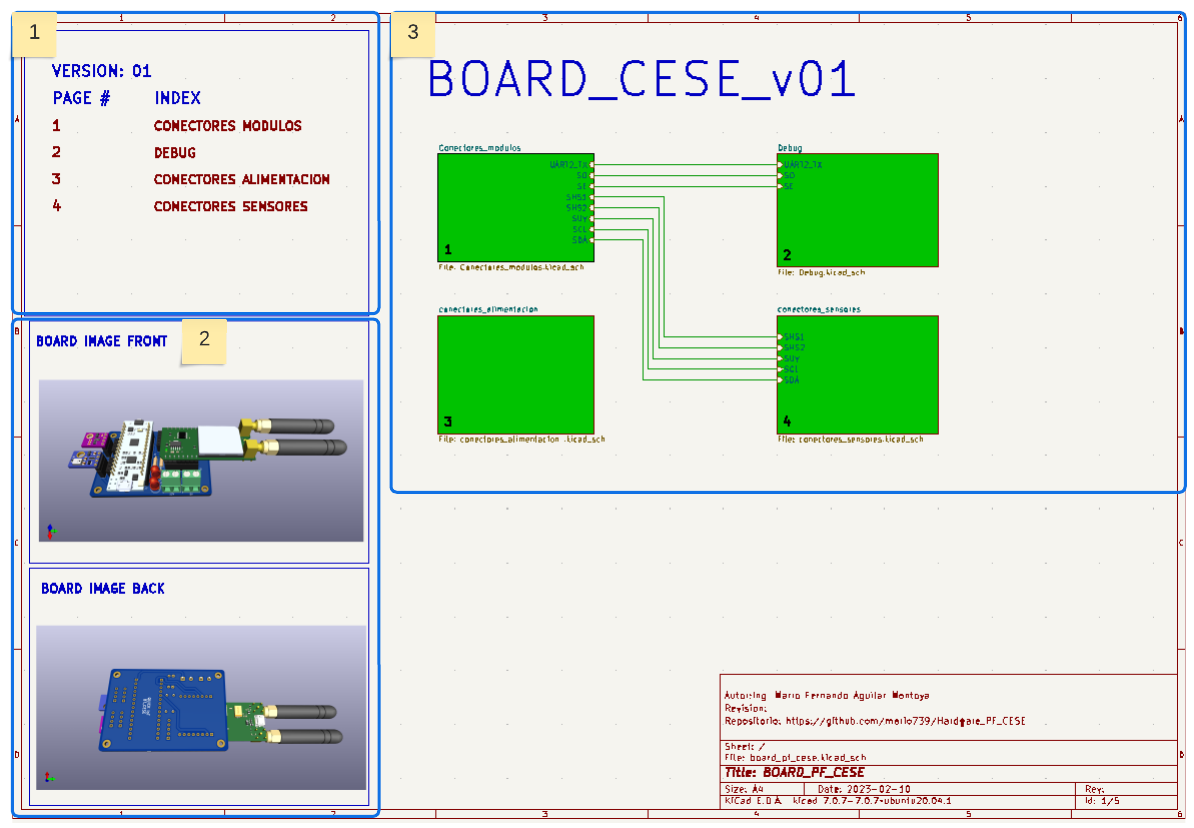
\includegraphics[width=\textwidth, height=8cm]{./Figures/esquematico_raiz.png}
	\caption{Esquemático página raíz.}
	\label{fig:esquematico root}
\end{figure}

En figura \ref{fig:esquematico modulos} se muestran los conectores de los módulos más importantes: el módulo de comunicación BG96, módulo NUCLEO-L432KC y la conexión entre ellos.

\begin{figure}[h]
  \centering
	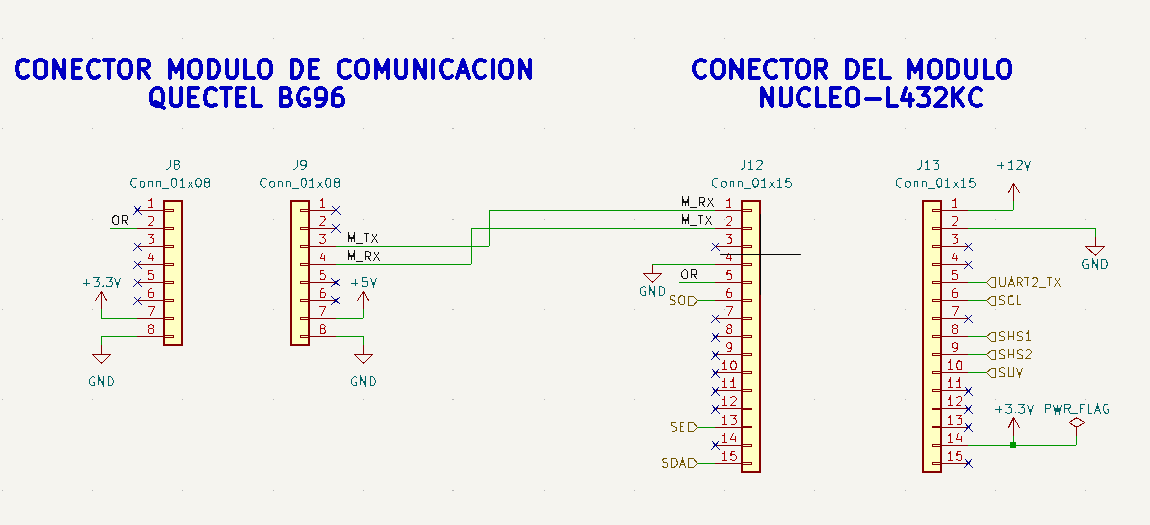
\includegraphics[width=10cm, height=4.5cm]{./Figures/esquematico_modulos.png}
	\caption{Conector módulo BG96 y NUCLEO-L432KC.}
	\label{fig:esquematico modulos}
\end{figure}

Se incorporaron dos leds con fines de depuración: uno para indicar si se logró la  conexión al servidor MQTT y el otro para señalar cualquier estado de error del sistema. También se incluyó un conector para un puerto serial a través del cual el módulo transmite las secuencias de comandos enviadas y recibidas del módulo de comunicación. En la \ref{fig:esquematico conectores de debug} se puede ver el circuito implementado.
\begin{figure}[h!]
  \centering
	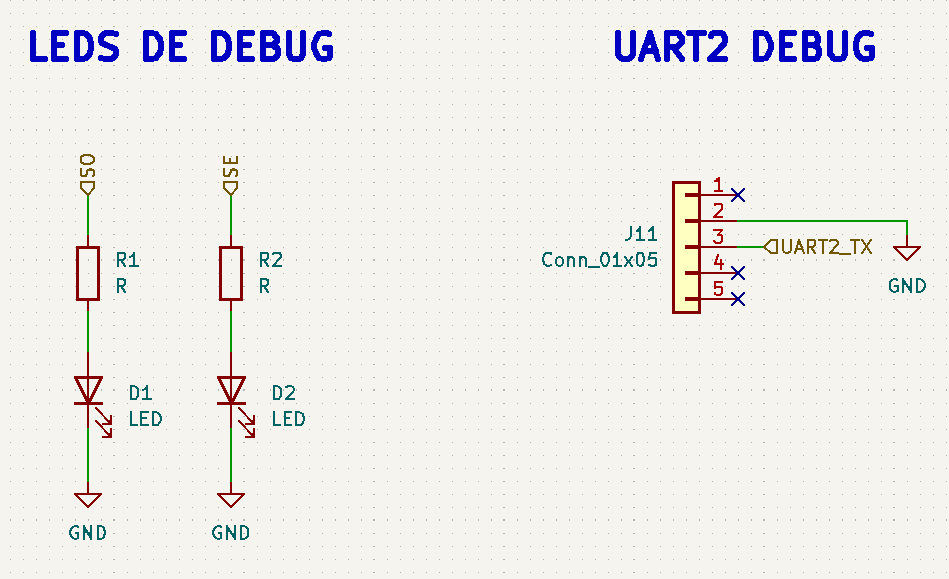
\includegraphics[width=10cm, height=3.5cm]{./Figures/esquematico_debug.png}
	\caption{Esquemático interfaz de debug.}
	\label{fig:esquematico conectores de debug}
\end{figure}

En la figura \ref{fig:esquematico conectores sensores} se pueden ver los conectores que se colocaron a la placa para conectar los sensores del nodo: sensor de humedad 1, sensor de humedad 2, sensor de luz UV y el sensor de humedad y temperatura ambiente AHT-10.
\begin{figure}[h!]
  \centering
	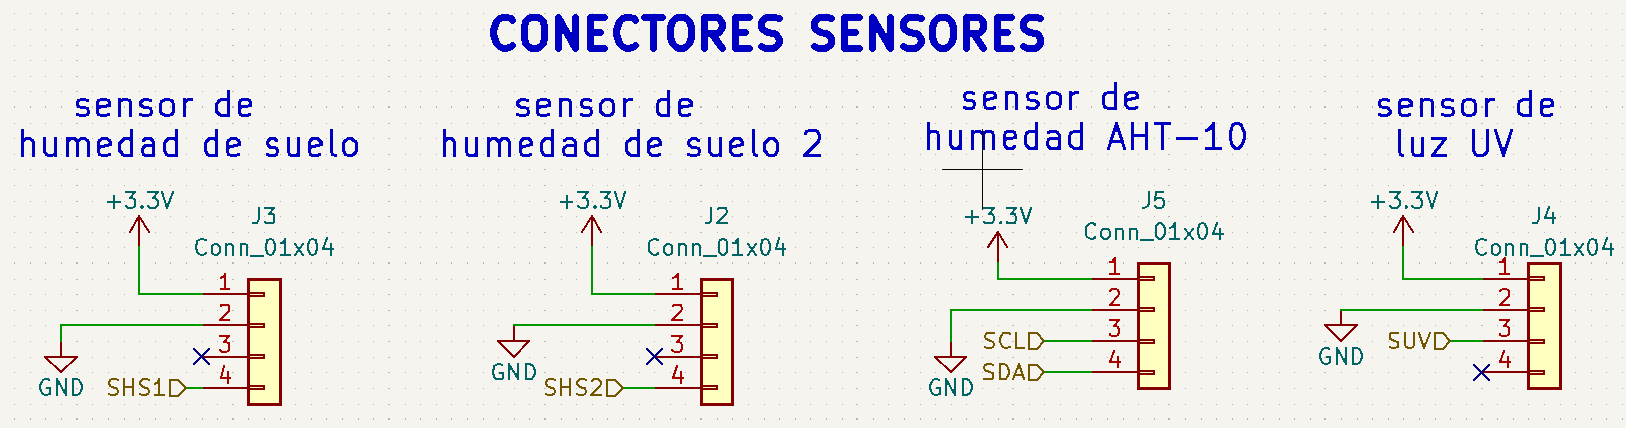
\includegraphics[width=10cm, height=4cm]{./Figures/conectores_sensores.png}
	\caption{Esquemático conectores sensores.}
	\label{fig:esquematico conectores sensores}
\end{figure}


Se colocaron dos colectores de alimentación como se muestra en la figura \ref{fig:esquematico conectores alimentacion}, el conector de 12V para alimentar al módulo del microcontrolador y el otro conector para alimentar al módulo de comunicación.
\begin{figure}[h!]
  \centering
	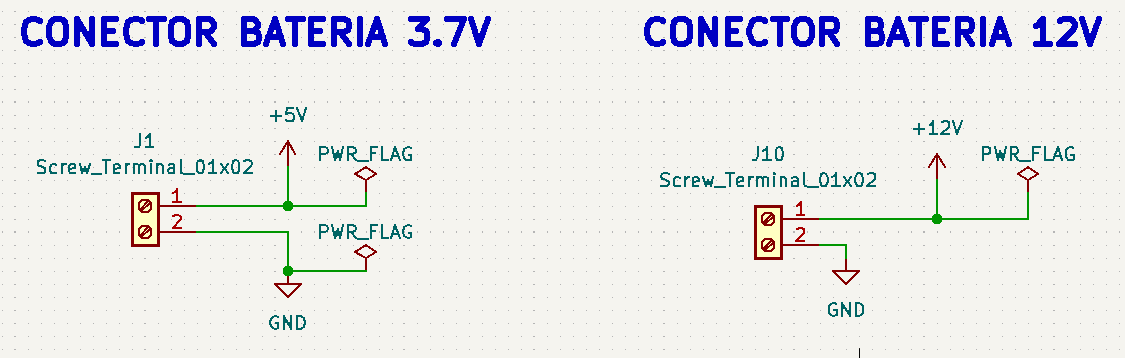
\includegraphics[width=10cm, height=3.5cm]{./Figures/esquematico_alimentacion.png}
	\caption{Esquemático conectores de alimentación.}
	\label{fig:esquematico conectores alimentacion}
\end{figure}

\subsection{PCB del hardware} 
La figura \ref{fig:PCB del proyecto} muestra el circuito impreso diseñado para el trabajo.

\begin{figure}[h!]
  \centering
  \begin{subfigure}[b]{0.28\linewidth}
  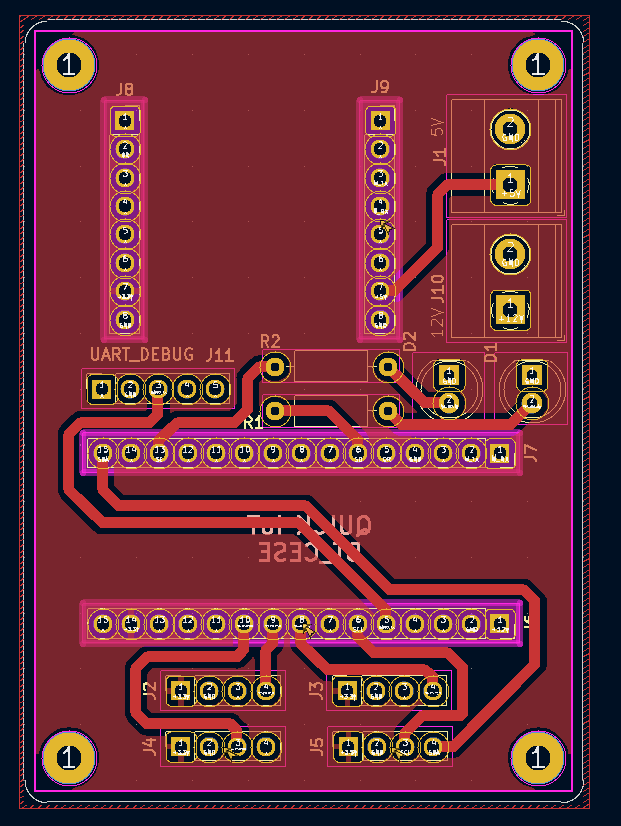
\includegraphics[width=\linewidth]{./Figures/pcb_top.png}
  \caption{Capa top PCB}
  \label{fig:Capa top PCB}
  \end{subfigure}
  \begin{subfigure}[b]{0.27\linewidth}
  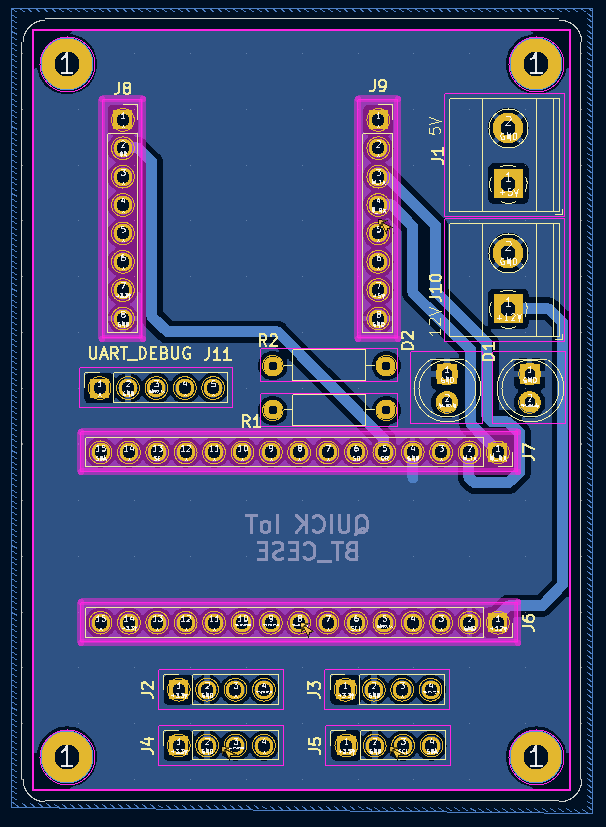
\includegraphics[width=\linewidth]{./Figures/pcb_bot.png}
  \caption{Capa bot PCB}
  \label{fig:Capa bot PCB}
  \end{subfigure}
  \caption{PCB del trabajo.}
  \label{fig:PCB del proyecto}
\end{figure}
\clearpage
En la figura \ref{fig:3D del modulo} se muestra el diseño de la tarjeta del circuito impreso en 3D.
\begin{figure}[h!]
  \centering
	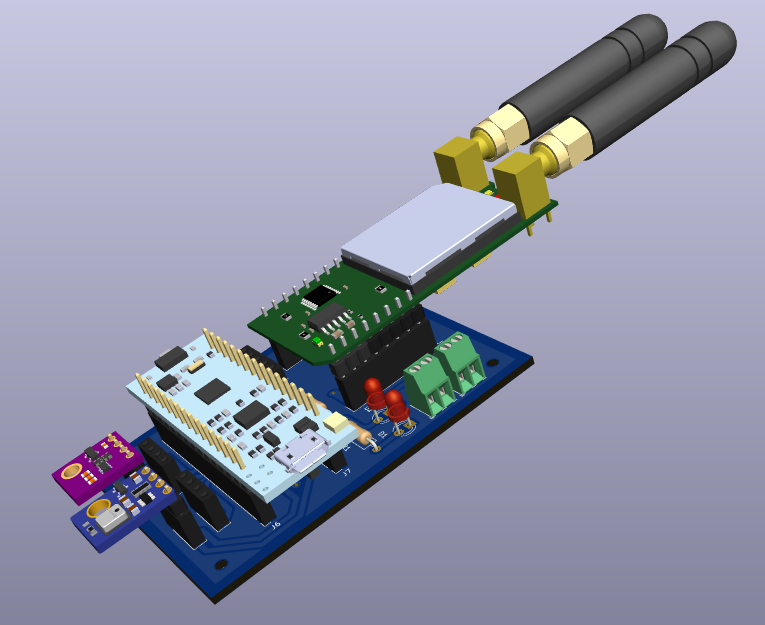
\includegraphics[width=7cm, height=4cm]{./Figures/tarjeta3d.png}
  \caption{Modelo 3D de la tarjeta.}
	\label{fig:3D del modulo}
\end{figure}
\subsection{Fabricación del circuito impreso} 
Una vez completado y validado el diseño, se generaron los archivos de fabricación y se mandaron a la empresa JLCPCB para su producción. La figura \ref{fig:PCB ensamblado} muestra la tarjeta ya ensamblada con los módulos. 
\begin{figure}[h!]
  \centering
	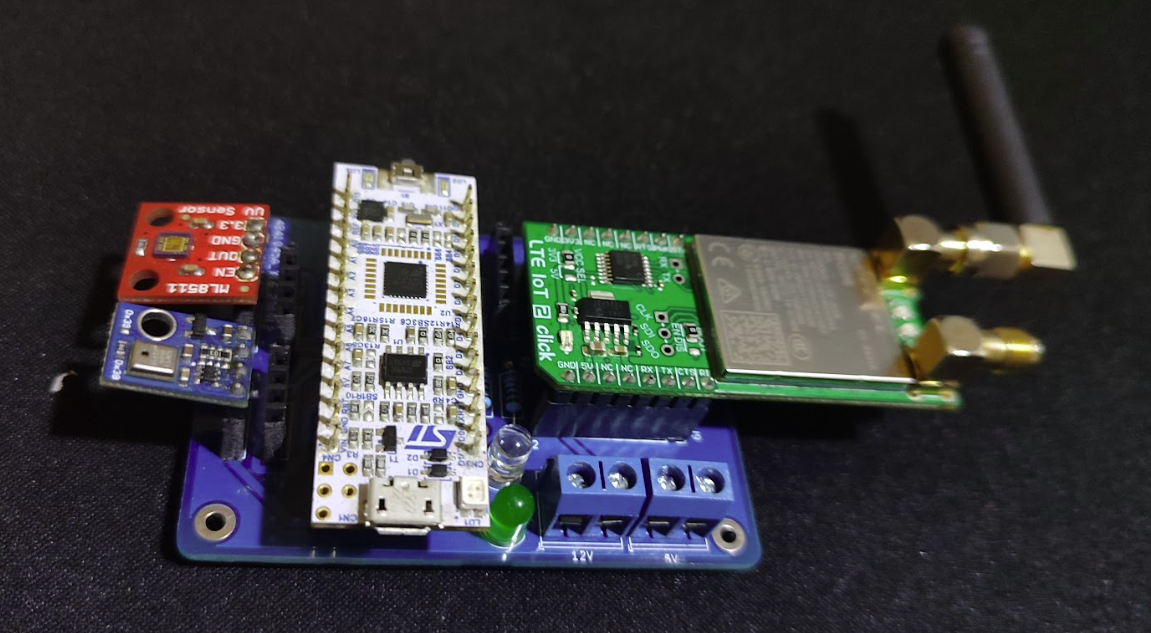
\includegraphics[width=7cm, height=4cm]{./Figures/hardware_vistalateral.png}
  \caption{PCB ensamblado.}
	\label{fig:PCB ensamblado}
\end{figure}

\section{Paneles de visualización}
La herramienta de visualización de ThingsBoard es muy versátil para el armado de paneles de visualización escalables y altamente configurables.

Se armó un panel de visualización principal que muestra los nodos sensores monitoreados por el sistema y un panel secundario que muestra las variables monitoreadas por cada nodo sensor a través de gráfica, tablas, etc.

\subsection{Panel principal} 
La figura \ref{fig:Panel principal} muestra el panel principal de la interfaz gráfica. A continuación, se detallarán las distintas áreas que componen este panel. Este se divide en las siguientes zonas:

\begin{itemize}
  \item Zona 1: listado de todos los nodos sensores implementados y activos, haciendo click en el sensor se navega al panel de visualización secundario.
  \item Zona 2: gráficas que representan la evolución en el tiempo de los valores de las variables registradas por los sensores.
  \item Zona 3: mapa con la ubicación de los nodos sensores implementados.
\end{itemize}

\begin{figure}[h]
  \centering
	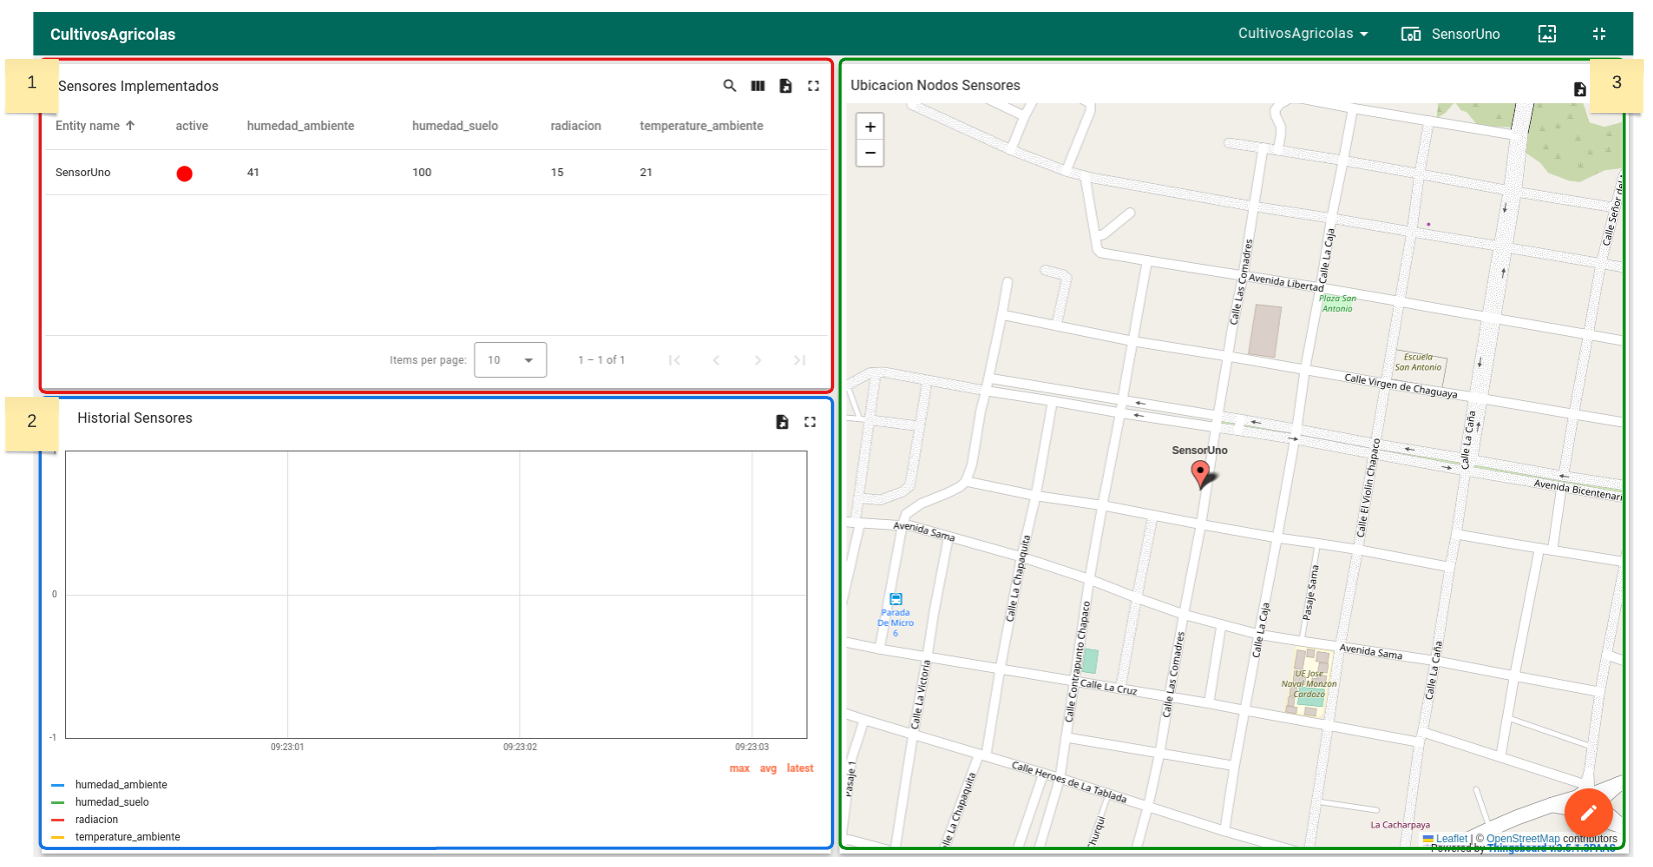
\includegraphics[width=\textwidth, height=7.5cm]{./Figures/panel_principal_editado.png}
  \caption{Panel principal de la interfaz gráfica.}
	\label{fig:Panel principal}
\end{figure}

\subsection{Panel nodo sensor} 

Para tener un mayor detalle de todos los parámetros de monitoreo de cada nodo sensor se creó un panel secundario que se muestra en la figura \ref{fig:Panel nodo sensor}. El panel está dividido en las siguientes zonas:
\begin{itemize}
  \item Zona 1: gráficas que muestran los cambios que van teniendo los valores de las variables medidas por los sensores con respecto al tiempo.
  \item Zona 2: widgets que muestran el último valor obtenido por el nodo sensor de cada variable monitoreada.
  \item Zona 3: tabla que muestra las alarmas que se activaron. 
  \item Zona 4: se tiene un mapa que muestra la ubicación del nodo sensor implementado.
\end{itemize}

\begin{figure}[htb!]
  \centering
	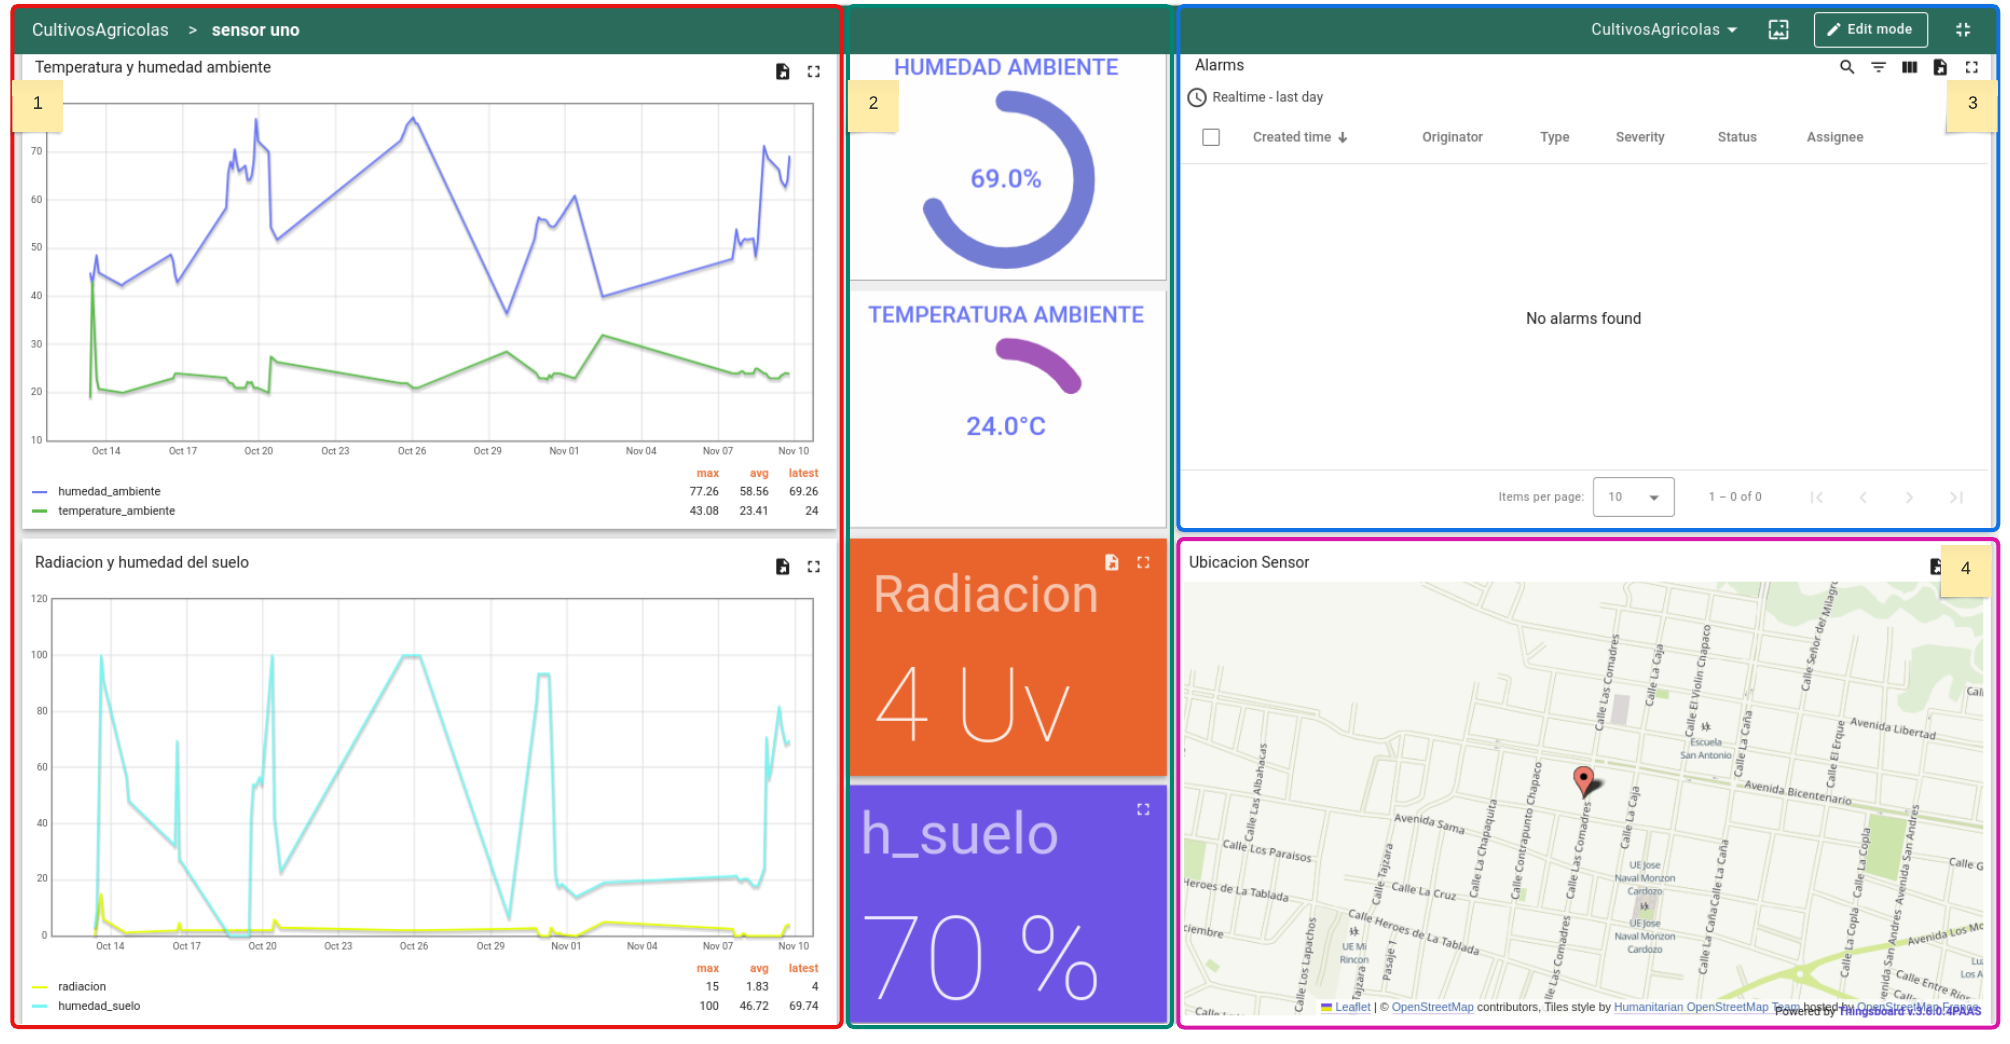
\includegraphics[width=\textwidth, height=7.5cm]{./Figures/panel_nodosensor_editado2.png}
  \caption{Panel nodo sensor.}
	\label{fig:Panel nodo sensor}
\end{figure}